\chapter{Working with Virtual Machines}

	\section{Introducing KVM Virtualization}
There are some basic requirements for KVM Virtualization on a server: 

\subsection{CPU Virtualization Support}
The CPU needs to be capable to support virtualization. This can be easily verified using the command:

\vspace{-15pt}
\begin{minted}{console}
# grep -E "vmx|svm" /proc/cpuinfo
\end{minted}
\vspace{-10pt}

\noindent
The presence of the \verb|vmx| flag is the indication that the CPU supports Intel's VT-x virtualization. However, for AMD processors, the equivalent is \verb|svm| indicating the presence of AMD's SVM technology. 

If the processor does in fact support virtualization, then the Linux Kernel can load the \verb|kvm| and the \verb|kvm-intel| or \verb|kvm-amd| modules. On top of the kernel lies the \textbf{libvirtd} daemon, which allow us to manage the KVM virtualization. It can also communicate other virtualization as well, such as Linux containers. 

\begin{figure}[H]
	\centering
	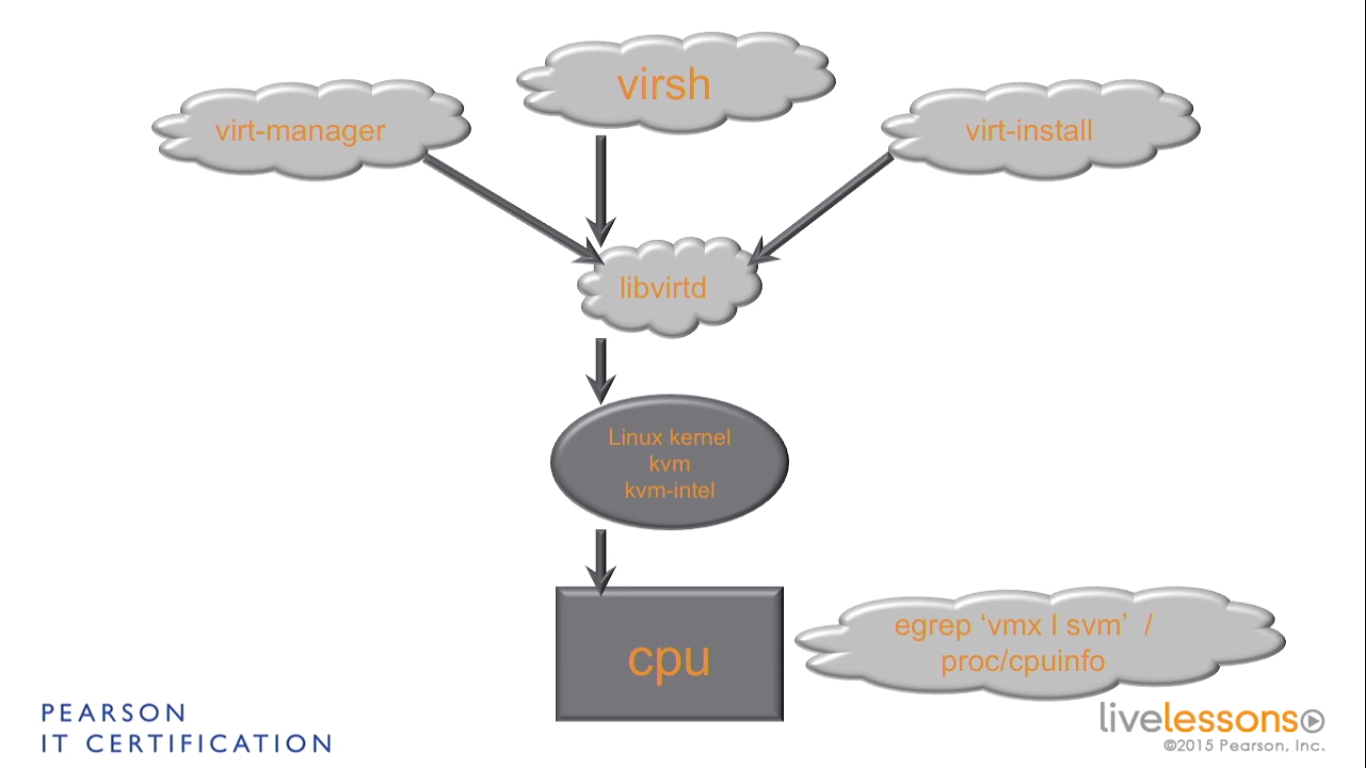
\includegraphics[width=0.9\linewidth]{Mod2/chapters/2.12.a}
	\caption{Virtualization}
	\label{fig:2 Virtualization}
\end{figure}


\verb|libvirtd| only serves as a generic interface to virtualization that can be used by other management programs such as \textbf{virt-manager}, which is a GUI based VM management tool. There's also \textbf{virsh}, a shell-based VM manager, that is extremely useful to manage multiple VMs in an automated way! 

There is also \verb|vert-install|, a small installation interface that allow us to install VMs. 

	\section{Managing Libvirt and KVM}
First we need to verify that the required kernel modules for KVM are available. This can be done with:

\vspace{-15pt}
\begin{minted}{console}
# lsmod | grep kvm
kvm_intel             200704  0
kvm                   585728  1 kvm_intel
irqbypass              16384  1 kvm
\end{minted}
\vspace{-10pt}

\noindent
The \verb|lsmod| command shows us the status of the Linux Kernel modules. The \verb|kvm| module is the generic KVM support module, while the \verb|kvm-intel| module provides platform specific support for KVM virtualization. 

Finally, we check if the \verb|libvirtd| daemon is up and running using:

\vspace{-15pt}
\begin{minted}{console}
# systemctl status libvirtd
libvirtd.service - Virtualization daemon
Loaded: loaded (/usr/lib/systemd/system/libvirtd.service; enabled; vendor pre
Active: active (running) since Sat 2017-12-02 16:08:39 IST; 2h 43min ago
Docs: man:libvirtd(8)
http://libvirt.org
Main PID: 945 (libvirtd)
Tasks: 18 (limit: 32768)
CGroup: /system.slice/libvirtd.service
945 /usr/sbin/libvirtd
1210 /usr/sbin/dnsmasq --conf-file=/var/lib/libvirt/dnsmasq/default
1211 /usr/sbin/dnsmasq --conf-file=/var/lib/libvirt/dnsmasq/default

Dec 02 16:08:55 lappyPrime dnsmasq[1210]: compile time options: IPv6 GNU-getopt 
Dec 02 16:08:55 lappyPrime dnsmasq-dhcp[1210]: DHCP, IP range 192.168.124.2 -- 1
Dec 02 16:08:55 lappyPrime dnsmasq-dhcp[1210]: DHCP, sockets bound exclusively t
Dec 02 16:08:55 lappyPrime dnsmasq[1210]: no servers found in /etc/resolv.conf, 
Dec 02 16:08:55 lappyPrime dnsmasq[1210]: read /etc/hosts - 2 addresses
Dec 02 16:08:55 lappyPrime dnsmasq[1210]: read /var/lib/libvirt/dnsmasq/default.
Dec 02 16:08:55 lappyPrime dnsmasq-dhcp[1210]: read /var/lib/libvirt/dnsmasq/def
Dec 02 16:09:37 lappyPrime dnsmasq[1210]: reading /etc/resolv.conf
Dec 02 16:09:37 lappyPrime dnsmasq[1210]: using nameserver 8.8.8.8#53
Dec 02 16:09:37 lappyPrime dnsmasq[1210]: using nameserver 202.38.180.7#53
\end{minted}
\vspace{-10pt}

Thus, this machine is completely ready for virtualization! If we run the \verb|ip link show| command, we can also find a virtual bridge called virbr0, which is provided courtesy of KVM. This network acts as if it's connected to a virtual switch and provides inter-VM bridged networking support. 

\vspace{-15pt}
\begin{minted}{console}
# ip link show
1: lo: <LOOPBACK,UP,LOWER_UP> mtu 65536 qdisc noqueue state UNKNOWN mode DEFAULT group default qlen 1000
link/loopback 00:00:00:00:00:00 brd 00:00:00:00:00:00
2: enp1s0: <NO-CARRIER,BROADCAST,MULTICAST,UP> mtu 1500 qdisc fq_codel state DOWN mode DEFAULT group default qlen 1000
link/ether 3c:52:82:b9:05:5f brd ff:ff:ff:ff:ff:ff
3: wlo1: <BROADCAST,MULTICAST,UP,LOWER_UP> mtu 1500 qdisc mq state UP mode DORMANT group default qlen 1000
link/ether 3c:95:09:de:4e:8d brd ff:ff:ff:ff:ff:ff
4: virbr0: <NO-CARRIER,BROADCAST,MULTICAST,UP> mtu 1500 qdisc noqueue state DOWN mode DEFAULT group default qlen 1000
link/ether 52:54:00:62:77:f7 brd ff:ff:ff:ff:ff:ff
5: virbr0-nic: <BROADCAST,MULTICAST> mtu 1500 qdisc fq_codel master virbr0 state DOWN mode DEFAULT group default qlen 1000
link/ether 52:54:00:62:77:f7 brd ff:ff:ff:ff:ff:ff
\end{minted}
\vspace{-10pt}

	\section{Using virsh}
KVM requires a 64-bit architecture host. This can be verified by using:

\vspace{-15pt}
\begin{minted}{console}
# arch
x86_64
\end{minted}
\vspace{-10pt}

\noindent
The \verb|x86_64| output tells us that the installed OS is 64-bit. The Virtualization shell is opened by simply typing \verb|virsh| which in turn supports a lot of commands. 

\vspace{-15pt}
\begin{minted}{console}
# virsh
Welcome to virsh, the virtualization interactive terminal.

Type:  'help' for help with commands
'quit' to quit

virsh # 
\end{minted}
\vspace{-10pt}

\subsection{Virsh commands}
\subsubsection{virsh list}
\vspace{-10pt}
The following are the \verb|virsh list| commands. They need to be run from the CLI directly. If the commands are being run from within the sub-shell provided by \verb|virsh| then only the second command onward suffices (i.e., virsh need not be retyped). 

\noindent
\begin{tabular}{lM{0.64}}
	\toprule
	\textbf{Command} &\textbf{Description} \\
	\midrule
	\textbf{virsh list} &Shows all the virtual machines that are currently running \\
	\textbf{virsh list all} &Shows all virtual machines that exist \\
	\textbf{virsh destroy <vmName>} &Merely pulls the plug on the VM, i.e., immediately terminates the running VM. \\
	\textbf{virsh start <vmName>} &Starts the VM. \\
	\bottomrule
\end{tabular}

\noindent
Each virtual machine on the system has a configuration file that defines what the VM consists of. The \verb|/etc/libvirt/| folder is related to the configuration of the \verb|libvirtd| daemon that acts as a common interface for all KVM managers. Inside it is a directory called \verb|qemu|. \textbf{qemu} is an old emulator that has been adapted for use in the KVM environment. The qemu configuration files are stored in this \verb|/etc/libvirt/qemu| directory in XML format. This file is auto-generated by virsh, and thus should only be edited with \verb|virsh edit <vmName>|. This has the benefit of ensuring nothing else is concurrently editing the file. 

	\section{Using virt-manager}
The \verb|virt-manager| is a GUI interface for the control of VMs. It can be started by:

\vspace{-15pt}
\begin{minted}{console}
# virt-manager
\end{minted}
\vspace{-10pt}

\noindent
Note that to control VMs made using \verb|virt-manager| from within \verb|virsh|, we need to be logged in under the same user when starting these utilities. They use the same libvirt database of VMs, but the user context can cause the VMs to be unavailable to some users!